\documentclass[1p]{elsarticle_modified}
%\bibliographystyle{elsarticle-num}

%\usepackage[colorlinks]{hyperref}
%\usepackage{abbrmath_seonhwa} %\Abb, \Ascr, \Acal ,\Abf, \Afrak
\usepackage{amsfonts}
\usepackage{amssymb}
\usepackage{amsmath}
\usepackage{amsthm}
\usepackage{scalefnt}
\usepackage{amsbsy}
\usepackage{kotex}
\usepackage{caption}
\usepackage{subfig}
\usepackage{color}
\usepackage{graphicx}
\usepackage{xcolor} %% white, black, red, green, blue, cyan, magenta, yellow
\usepackage{float}
\usepackage{setspace}
\usepackage{hyperref}

\usepackage{tikz}
\usetikzlibrary{arrows}

\usepackage{multirow}
\usepackage{array} % fixed length table
\usepackage{hhline}

%%%%%%%%%%%%%%%%%%%%%
\makeatletter
\renewcommand*\env@matrix[1][\arraystretch]{%
	\edef\arraystretch{#1}%
	\hskip -\arraycolsep
	\let\@ifnextchar\new@ifnextchar
	\array{*\c@MaxMatrixCols c}}
\makeatother %https://tex.stackexchange.com/questions/14071/how-can-i-increase-the-line-spacing-in-a-matrix
%%%%%%%%%%%%%%%

\usepackage[normalem]{ulem}

\newcommand{\msout}[1]{\ifmmode\text{\sout{\ensuremath{#1}}}\else\sout{#1}\fi}
%SOURCE: \msout is \stkout macro in https://tex.stackexchange.com/questions/20609/strikeout-in-math-mode

\newcommand{\cancel}[1]{
	\ifmmode
	{\color{red}\msout{#1}}
	\else
	{\color{red}\sout{#1}}
	\fi
}

\newcommand{\add}[1]{
	{\color{blue}\uwave{#1}}
}

\newcommand{\replace}[2]{
	\ifmmode
	{\color{red}\msout{#1}}{\color{blue}\uwave{#2}}
	\else
	{\color{red}\sout{#1}}{\color{blue}\uwave{#2}}
	\fi
}

\newcommand{\Sol}{\mathcal{S}} %segment
\newcommand{\D}{D} %diagram
\newcommand{\A}{\mathcal{A}} %arc


%%%%%%%%%%%%%%%%%%%%%%%%%%%%%5 test

\def\sl{\operatorname{\textup{SL}}(2,\Cbb)}
\def\psl{\operatorname{\textup{PSL}}(2,\Cbb)}
\def\quan{\mkern 1mu \triangleright \mkern 1mu}

\theoremstyle{definition}
\newtheorem{thm}{Theorem}[section]
\newtheorem{prop}[thm]{Proposition}
\newtheorem{lem}[thm]{Lemma}
\newtheorem{ques}[thm]{Question}
\newtheorem{cor}[thm]{Corollary}
\newtheorem{defn}[thm]{Definition}
\newtheorem{exam}[thm]{Example}
\newtheorem{rmk}[thm]{Remark}
\newtheorem{alg}[thm]{Algorithm}

\newcommand{\I}{\sqrt{-1}}
\begin{document}

%\begin{frontmatter}
%
%\title{Boundary parabolic representations of knots up to 8 crossings}
%
%%% Group authors per affiliation:
%\author{Yunhi Cho} 
%\address{Department of Mathematics, University of Seoul, Seoul, Korea}
%\ead{yhcho@uos.ac.kr}
%
%
%\author{Seonhwa Kim} %\fnref{s_kim}}
%\address{Center for Geometry and Physics, Institute for Basic Science, Pohang, 37673, Korea}
%\ead{ryeona17@ibs.re.kr}
%
%\author{Hyuk Kim}
%\address{Department of Mathematical Sciences, Seoul National University, Seoul 08826, Korea}
%\ead{hyukkim@snu.ac.kr}
%
%\author{Seokbeom Yoon}
%\address{Department of Mathematical Sciences, Seoul National University, Seoul, 08826,  Korea}
%\ead{sbyoon15@snu.ac.kr}
%
%\begin{abstract}
%We find all boundary parabolic representation of knots up to 8 crossings.
%
%\end{abstract}
%\begin{keyword}
%    \MSC[2010] 57M25 
%\end{keyword}
%
%\end{frontmatter}

%\linenumbers
%\tableofcontents
%
\newcommand\colored[1]{\textcolor{white}{\rule[-0.35ex]{0.8em}{1.4ex}}\kern-0.8em\color{red} #1}%
%\newcommand\colored[1]{\textcolor{white}{ #1}\kern-2.17ex	\textcolor{white}{ #1}\kern-1.81ex	\textcolor{white}{ #1}\kern-2.15ex\color{red}#1	}

{\Large $\underline{12n_{0879}~(K12n_{0879})}$}

\setlength{\tabcolsep}{10pt}
\renewcommand{\arraystretch}{1.6}
\vspace{1cm}\begin{tabular}{m{100pt}>{\centering\arraybackslash}m{274pt}}
\multirow{5}{120pt}{
	\centering
	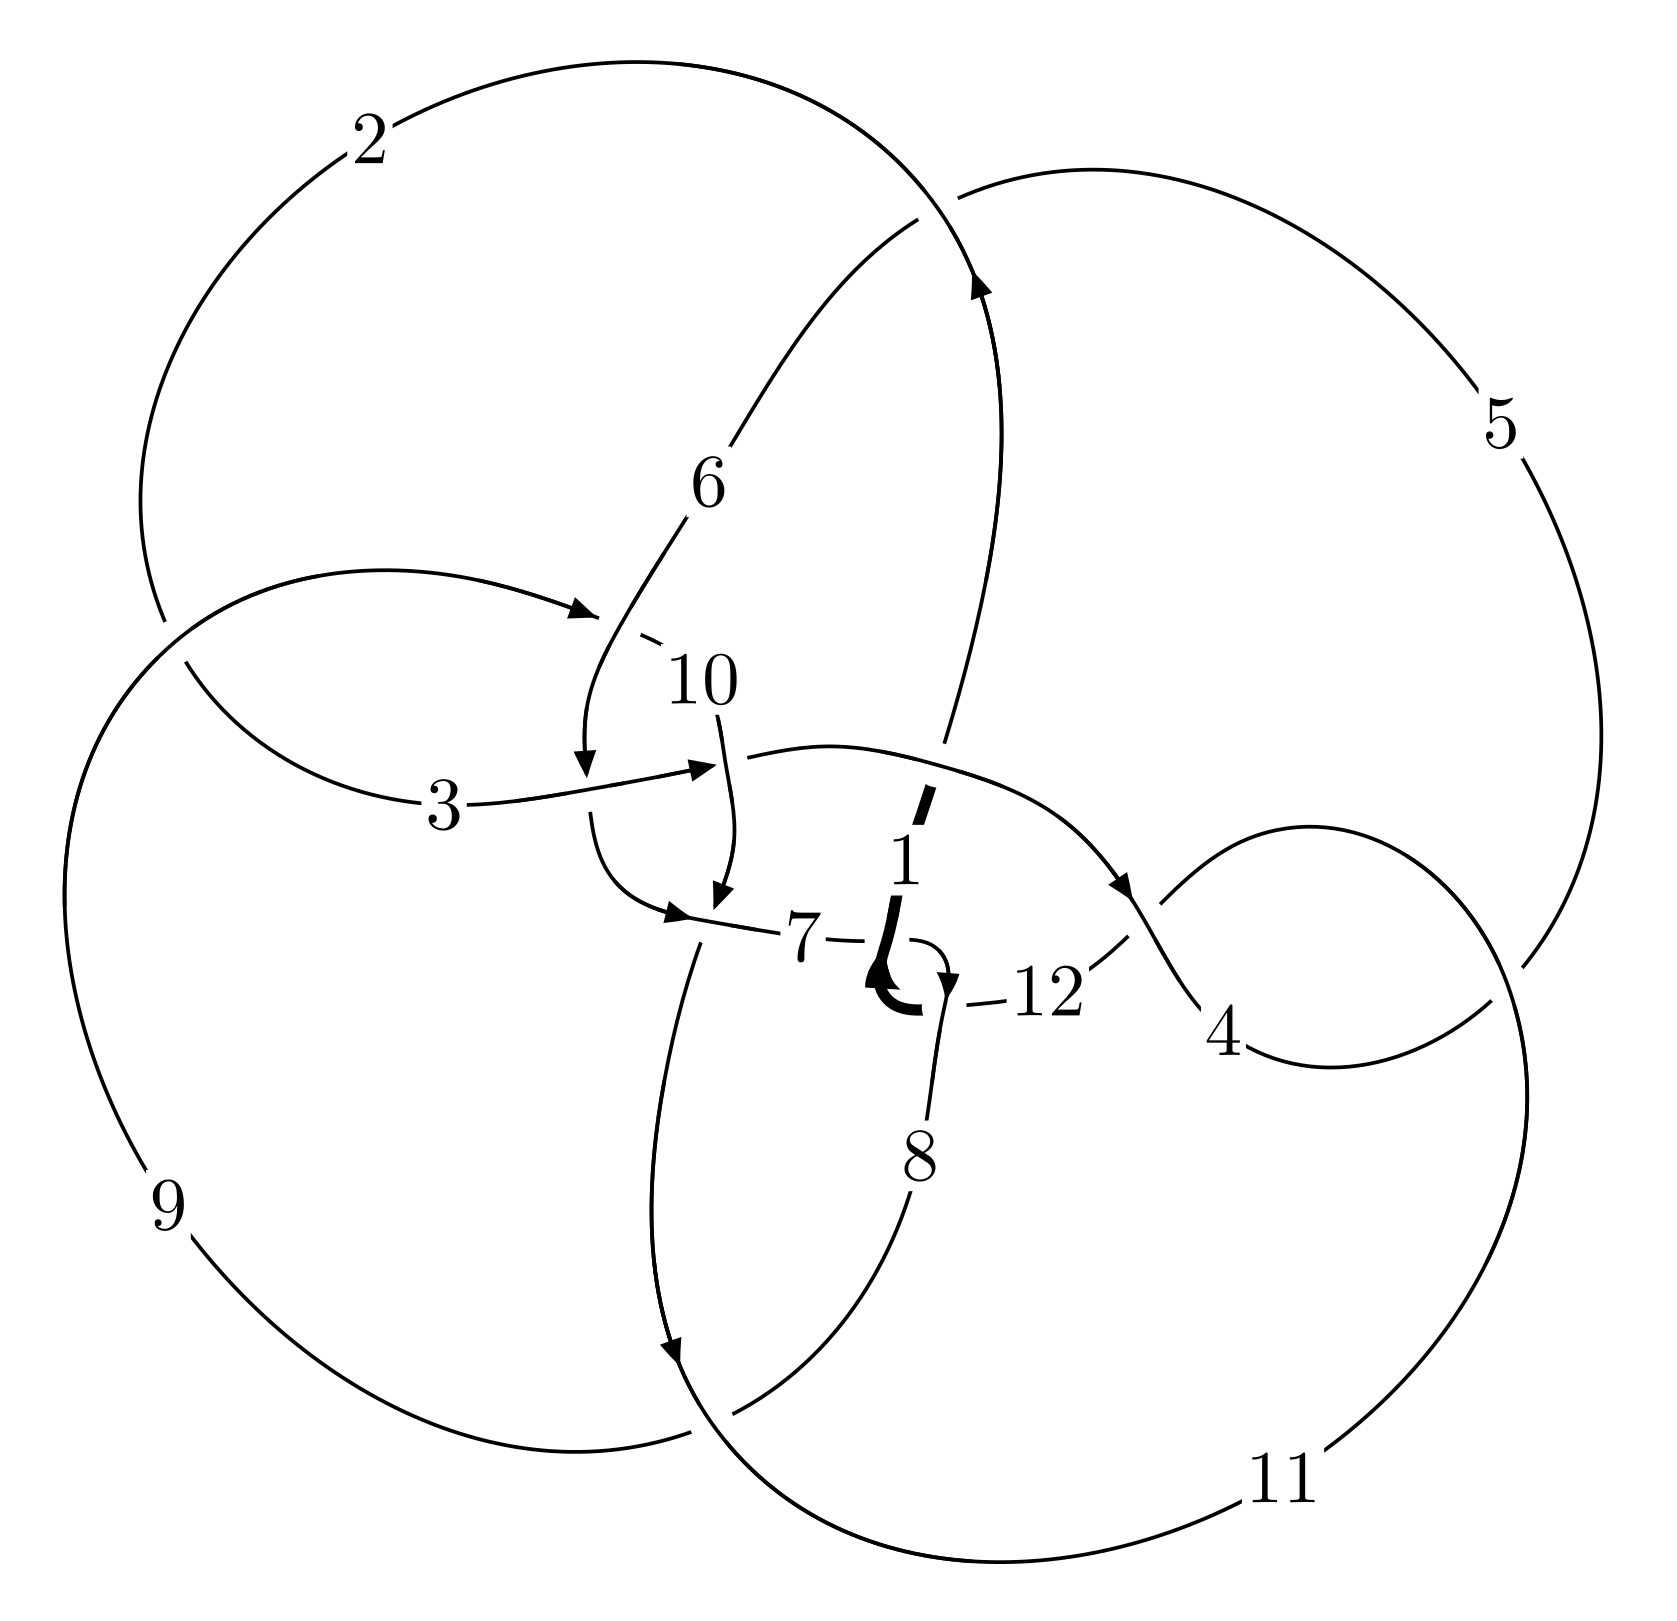
\includegraphics[width=112pt]{../../../GIT/diagram.site/Diagrams/png/2968_12n_0879.png}\\
\ \ \ A knot diagram\footnotemark}&
\allowdisplaybreaks
\textbf{Linearized knot diagam} \\
\cline{2-2}
 &
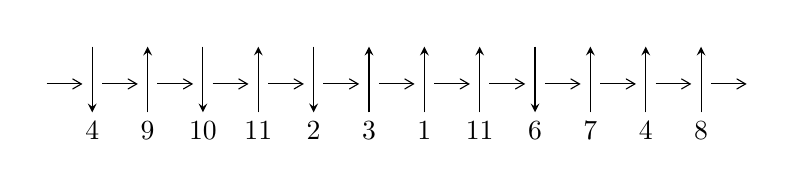
\begin{tikzpicture}[x=20pt, y=17pt]
	% nodes
	\node (C0) at (0, 0) {};
	\node (C1) at (1, 0) {};
	\node (C1U) at (1, +1) {};
	\node (C1D) at (1, -1) {4};

	\node (C2) at (2, 0) {};
	\node (C2U) at (2, +1) {};
	\node (C2D) at (2, -1) {9};

	\node (C3) at (3, 0) {};
	\node (C3U) at (3, +1) {};
	\node (C3D) at (3, -1) {10};

	\node (C4) at (4, 0) {};
	\node (C4U) at (4, +1) {};
	\node (C4D) at (4, -1) {11};

	\node (C5) at (5, 0) {};
	\node (C5U) at (5, +1) {};
	\node (C5D) at (5, -1) {2};

	\node (C6) at (6, 0) {};
	\node (C6U) at (6, +1) {};
	\node (C6D) at (6, -1) {3};

	\node (C7) at (7, 0) {};
	\node (C7U) at (7, +1) {};
	\node (C7D) at (7, -1) {1};

	\node (C8) at (8, 0) {};
	\node (C8U) at (8, +1) {};
	\node (C8D) at (8, -1) {11};

	\node (C9) at (9, 0) {};
	\node (C9U) at (9, +1) {};
	\node (C9D) at (9, -1) {6};

	\node (C10) at (10, 0) {};
	\node (C10U) at (10, +1) {};
	\node (C10D) at (10, -1) {7};

	\node (C11) at (11, 0) {};
	\node (C11U) at (11, +1) {};
	\node (C11D) at (11, -1) {4};

	\node (C12) at (12, 0) {};
	\node (C12U) at (12, +1) {};
	\node (C12D) at (12, -1) {8};
	\node (C13) at (13, 0) {};

	% arrows
	\draw[->,>={angle 60}]
	(C0) edge (C1) (C1) edge (C2) (C2) edge (C3) (C3) edge (C4) (C4) edge (C5) (C5) edge (C6) (C6) edge (C7) (C7) edge (C8) (C8) edge (C9) (C9) edge (C10) (C10) edge (C11) (C11) edge (C12) (C12) edge (C13) ;	\draw[->,>=stealth]
	(C1U) edge (C1D) (C2D) edge (C2U) (C3U) edge (C3D) (C4D) edge (C4U) (C5U) edge (C5D) (C6D) edge (C6U) (C7D) edge (C7U) (C8D) edge (C8U) (C9U) edge (C9D) (C10D) edge (C10U) (C11D) edge (C11U) (C12D) edge (C12U) ;
	\end{tikzpicture} \\
\hhline{~~} \\& 
\textbf{Solving Sequence} \\ \cline{2-2} 
 &
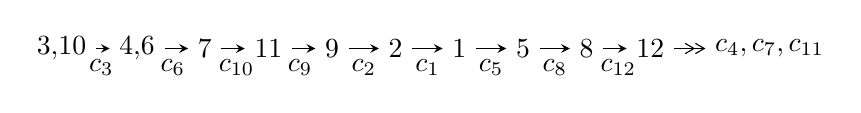
\begin{tikzpicture}[x=23pt, y=7pt]
	% node
	\node (A0) at (-1/8, 0) {3,10};
	\node (A1) at (17/16, 0) {4,6};
	\node (A2) at (17/8, 0) {7};
	\node (A3) at (25/8, 0) {11};
	\node (A4) at (33/8, 0) {9};
	\node (A5) at (41/8, 0) {2};
	\node (A6) at (49/8, 0) {1};
	\node (A7) at (57/8, 0) {5};
	\node (A8) at (65/8, 0) {8};
	\node (A9) at (73/8, 0) {12};
	\node (C1) at (1/2, -1) {$c_{3}$};
	\node (C2) at (13/8, -1) {$c_{6}$};
	\node (C3) at (21/8, -1) {$c_{10}$};
	\node (C4) at (29/8, -1) {$c_{9}$};
	\node (C5) at (37/8, -1) {$c_{2}$};
	\node (C6) at (45/8, -1) {$c_{1}$};
	\node (C7) at (53/8, -1) {$c_{5}$};
	\node (C8) at (61/8, -1) {$c_{8}$};
	\node (C9) at (69/8, -1) {$c_{12}$};
	\node (A10) at (11, 0) {$c_{4},c_{7},c_{11}$};

	% edge
	\draw[->,>=stealth]	
	(A0) edge (A1) (A1) edge (A2) (A2) edge (A3) (A3) edge (A4) (A4) edge (A5) (A5) edge (A6) (A6) edge (A7) (A7) edge (A8) (A8) edge (A9) ;
	\draw[->>,>={angle 60}]	
	(A9) edge (A10);
\end{tikzpicture} \\ 

\end{tabular} \\

\footnotetext{
The image of knot diagram is generated by the software ``\textbf{Draw programme}" developed by Andrew Bartholomew(\url{http://www.layer8.co.uk/maths/draw/index.htm\#Running-draw}), where we modified some parts for our purpose(\url{https://github.com/CATsTAILs/LinksPainter}).
}\phantom \\ \newline 
\centering \textbf{Ideals for irreducible components\footnotemark of $X_{\text{par}}$} 
 
\begin{align*}
I^u_{1}&=\langle 
2.18451\times10^{18} u^{23}-3.11362\times10^{18} u^{22}+\cdots+1.10562\times10^{17} b+1.21069\times10^{18},\;a-1,\\
\phantom{I^u_{1}}&\phantom{= \langle  }3 u^{24}-3 u^{23}+\cdots+u+1\rangle \\
I^u_{2}&=\langle 
2.45436\times10^{314} u^{67}-2.51900\times10^{313} u^{66}+\cdots+3.33912\times10^{315} b-2.97612\times10^{315},\\
\phantom{I^u_{2}}&\phantom{= \langle  }5.14656\times10^{314} u^{67}+3.56618\times10^{314} u^{66}+\cdots+6.67823\times10^{315} a-2.19657\times10^{315},\\
\phantom{I^u_{2}}&\phantom{= \langle  }8 u^{68}+40 u^{66}+\cdots-270 u+50\rangle \\
I^u_{3}&=\langle 
83485020528 u^{16}-39219382232 u^{15}+\cdots+2862203951 b+39645537732,\;a+1,\\
\phantom{I^u_{3}}&\phantom{= \langle  }4 u^{17}-4 u^{16}+\cdots+3 u-1\rangle \\
I^u_{4}&=\langle 
-18 u^3+24 u^2+b-21 u+8,\;-30 u^3+42 u^2+2 a-41 u+17,\;6 u^4-12 u^3+13 u^2-8 u+2\rangle \\
\\
\end{align*}
\raggedright * 4 irreducible components of $\dim_{\mathbb{C}}=0$, with total 113 representations.\\
\footnotetext{All coefficients of polynomials are rational numbers. But the coefficients are sometimes approximated in decimal forms when there is not enough margin.}
\newpage
\renewcommand{\arraystretch}{1}
\centering \section*{I. $I^u_{1}= \langle 2.18\times10^{18} u^{23}-3.11\times10^{18} u^{22}+\cdots+1.11\times10^{17} b+1.21\times10^{18},\;a-1,\;3 u^{24}-3 u^{23}+\cdots+u+1 \rangle$}
\flushleft \textbf{(i) Arc colorings}\\
\begin{tabular}{m{7pt} m{180pt} m{7pt} m{180pt} }
\flushright $a_{3}=$&$\begin{pmatrix}1\\0\end{pmatrix}$ \\
\flushright $a_{10}=$&$\begin{pmatrix}0\\u\end{pmatrix}$ \\
\flushright $a_{4}=$&$\begin{pmatrix}1\\u^2\end{pmatrix}$ \\
\flushright $a_{6}=$&$\begin{pmatrix}1\\-19.7583 u^{23}+28.1618 u^{22}+\cdots+11.4162 u-10.9504\end{pmatrix}$ \\
\flushright $a_{7}=$&$\begin{pmatrix}-19.7583 u^{23}+28.1618 u^{22}+\cdots+11.4162 u-9.95035\\-19.7583 u^{23}+28.1618 u^{22}+\cdots+11.4162 u-10.9504\end{pmatrix}$ \\
\flushright $a_{11}=$&$\begin{pmatrix}-3.47015 u^{23}+5.78314 u^{22}+\cdots-3.89407 u+1.41709\\-11.8736 u^{23}+19.3044 u^{22}+\cdots+0.470185 u-5.16901\end{pmatrix}$ \\
\flushright $a_{9}=$&$\begin{pmatrix}u\\8.40348 u^{23}-13.5213 u^{22}+\cdots-3.36425 u+6.58610\end{pmatrix}$ \\
\flushright $a_{2}=$&$\begin{pmatrix}-5.11782 u^{23}+8.44910 u^{22}+\cdots+3.78494 u-1.80116\\2.31299 u^{23}-4.48479 u^{22}+\cdots+2.57381 u+1.15672\end{pmatrix}$ \\
\flushright $a_{1}=$&$\begin{pmatrix}-0.316894 u^{23}-0.861176 u^{22}+\cdots+5.76323 u+0.465985\\5.20333 u^{23}-8.76032 u^{22}+\cdots+2.47662 u+2.65983\end{pmatrix}$ \\
\flushright $a_{5}=$&$\begin{pmatrix}-8.28934 u^{23}+7.65842 u^{22}+\cdots+6.46724 u-3.91525\\-27.1673 u^{23}+42.5966 u^{22}+\cdots+5.38232 u-13.8780\end{pmatrix}$ \\
\flushright $a_{8}=$&$\begin{pmatrix}-18.0653 u^{23}+25.7028 u^{22}+\cdots+5.14347 u-6.60098\\-18.6559 u^{23}+29.0833 u^{22}+\cdots+3.56041 u-6.94383\end{pmatrix}$ \\
\flushright $a_{12}=$&$\begin{pmatrix}13.1720 u^{23}-21.8361 u^{22}+\cdots+3.80961 u+2.98092\\17.5768 u^{23}-28.7733 u^{22}+\cdots-1.58709 u+7.28605\end{pmatrix}$\\&\end{tabular}
\flushleft \textbf{(ii) Obstruction class $= -1$}\\~\\
\flushleft \textbf{(iii) Cusp Shapes $= -\frac{10401411537800859069}{110561902854140359} u^{23}+\frac{17169214705690460772}{110561902854140359} u^{22}+\cdots+\frac{2497259999525294046}{110561902854140359} u-\frac{6190596405972712460}{110561902854140359}$}\\~\\
\newpage\renewcommand{\arraystretch}{1}
\flushleft \textbf{(iv) u-Polynomials at the component}\newline \\
\begin{tabular}{m{50pt}|m{274pt}}
Crossings & \hspace{64pt}u-Polynomials at each crossing \\
\hline $$\begin{aligned}c_{1}\end{aligned}$$&$\begin{aligned}
&3(3 u^{24}-3 u^{23}+\cdots-19 u+1)
\end{aligned}$\\
\hline $$\begin{aligned}c_{2},c_{10}\end{aligned}$$&$\begin{aligned}
&u^{24}+u^{23}+\cdots-3 u-3
\end{aligned}$\\
\hline $$\begin{aligned}c_{3},c_{9}\end{aligned}$$&$\begin{aligned}
&3(3 u^{24}+3 u^{23}+\cdots- u+1)
\end{aligned}$\\
\hline $$\begin{aligned}c_{4},c_{11}\end{aligned}$$&$\begin{aligned}
&3(3 u^{24}-3 u^{23}+\cdots+2 u+1)
\end{aligned}$\\
\hline $$\begin{aligned}c_{5}\end{aligned}$$&$\begin{aligned}
&u^{24}-3 u^{23}+\cdots-33 u+3
\end{aligned}$\\
\hline $$\begin{aligned}c_{6}\end{aligned}$$&$\begin{aligned}
&u^{24}-17 u^{23}+\cdots+448 u-64
\end{aligned}$\\
\hline $$\begin{aligned}c_{7},c_{12}\end{aligned}$$&$\begin{aligned}
&u^{24}-11 u^{23}+\cdots-192 u+32
\end{aligned}$\\
\hline $$\begin{aligned}c_{8}\end{aligned}$$&$\begin{aligned}
&9(9 u^{24}+168 u^{23}+\cdots-30720 u-4096)
\end{aligned}$\\
\hline
\end{tabular}\\~\\
\newpage\renewcommand{\arraystretch}{1}
\flushleft \textbf{(v) Riley Polynomials at the component}\newline \\
\begin{tabular}{m{50pt}|m{274pt}}
Crossings & \hspace{64pt}Riley Polynomials at each crossing \\
\hline $$\begin{aligned}c_{1}\end{aligned}$$&$\begin{aligned}
&9(9 y^{24}+201 y^{23}+\cdots-165 y+1)
\end{aligned}$\\
\hline $$\begin{aligned}c_{2},c_{10}\end{aligned}$$&$\begin{aligned}
&y^{24}-5 y^{23}+\cdots+21 y+9
\end{aligned}$\\
\hline $$\begin{aligned}c_{3},c_{9}\end{aligned}$$&$\begin{aligned}
&9(9 y^{24}-51 y^{23}+\cdots-17 y+1)
\end{aligned}$\\
\hline $$\begin{aligned}c_{4},c_{11}\end{aligned}$$&$\begin{aligned}
&9(9 y^{24}-267 y^{23}+\cdots-18 y+1)
\end{aligned}$\\
\hline $$\begin{aligned}c_{5}\end{aligned}$$&$\begin{aligned}
&y^{24}+11 y^{23}+\cdots-69 y+9
\end{aligned}$\\
\hline $$\begin{aligned}c_{6}\end{aligned}$$&$\begin{aligned}
&y^{24}+7 y^{23}+\cdots-36864 y+4096
\end{aligned}$\\
\hline $$\begin{aligned}c_{7},c_{12}\end{aligned}$$&$\begin{aligned}
&y^{24}+9 y^{23}+\cdots+4608 y+1024
\end{aligned}$\\
\hline $$\begin{aligned}c_{8}\end{aligned}$$&$\begin{aligned}
&81(81 y^{24}-558 y^{23}+\cdots-4.40402\times10^{7} y+1.67772\times10^{7})
\end{aligned}$\\
\hline
\end{tabular}\\~\\
\newpage\flushleft \textbf{(vi) Complex Volumes and Cusp Shapes}
$$\begin{array}{c|c|c}  
\text{Solutions to }I^u_{1}& \I (\text{vol} + \sqrt{-1}CS) & \text{Cusp shape}\\
 \hline 
\begin{aligned}
u &= \phantom{-}0.532676 + 0.913923 I \\
a &= \phantom{-}1.00000\phantom{ +0.000000I} \\
b &= -0.790735 + 0.557429 I\end{aligned}
 & \phantom{-}0.60856 - 1.63023 I & \phantom{-}4.46172 + 2.19213 I \\ \hline\begin{aligned}
u &= \phantom{-}0.532676 - 0.913923 I \\
a &= \phantom{-}1.00000\phantom{ +0.000000I} \\
b &= -0.790735 - 0.557429 I\end{aligned}
 & \phantom{-}0.60856 + 1.63023 I & \phantom{-}4.46172 - 2.19213 I \\ \hline\begin{aligned}
u &= -0.706049 + 0.814568 I \\
a &= \phantom{-}1.00000\phantom{ +0.000000I} \\
b &= -1.19229 - 0.96975 I\end{aligned}
 & \phantom{-}3.12317 + 4.41220 I & \phantom{-}8.88741 - 6.41775 I \\ \hline\begin{aligned}
u &= -0.706049 - 0.814568 I \\
a &= \phantom{-}1.00000\phantom{ +0.000000I} \\
b &= -1.19229 + 0.96975 I\end{aligned}
 & \phantom{-}3.12317 - 4.41220 I & \phantom{-}8.88741 + 6.41775 I \\ \hline\begin{aligned}
u &= \phantom{-}1.077440 + 0.425171 I \\
a &= \phantom{-}1.00000\phantom{ +0.000000I} \\
b &= -0.372534 + 0.567998 I\end{aligned}
 & \phantom{-}0.51482 - 4.14942 I & \phantom{-}0.15057 + 3.98630 I \\ \hline\begin{aligned}
u &= \phantom{-}1.077440 - 0.425171 I \\
a &= \phantom{-}1.00000\phantom{ +0.000000I} \\
b &= -0.372534 - 0.567998 I\end{aligned}
 & \phantom{-}0.51482 + 4.14942 I & \phantom{-}0.15057 - 3.98630 I \\ \hline\begin{aligned}
u &= \phantom{-}0.799855 + 0.085298 I \\
a &= \phantom{-}1.00000\phantom{ +0.000000I} \\
b &= \phantom{-}0.479827 + 0.465785 I\end{aligned}
 & -2.57731 + 3.83319 I & \phantom{-}9.74735 - 1.51258 I \\ \hline\begin{aligned}
u &= \phantom{-}0.799855 - 0.085298 I \\
a &= \phantom{-}1.00000\phantom{ +0.000000I} \\
b &= \phantom{-}0.479827 - 0.465785 I\end{aligned}
 & -2.57731 - 3.83319 I & \phantom{-}9.74735 + 1.51258 I \\ \hline\begin{aligned}
u &= \phantom{-}0.968057 + 0.775960 I \\
a &= \phantom{-}1.00000\phantom{ +0.000000I} \\
b &= -1.25250 + 1.11203 I\end{aligned}
 & -2.68123 - 8.44569 I & \phantom{-}4.87208 + 6.96290 I \\ \hline\begin{aligned}
u &= \phantom{-}0.968057 - 0.775960 I \\
a &= \phantom{-}1.00000\phantom{ +0.000000I} \\
b &= -1.25250 - 1.11203 I\end{aligned}
 & -2.68123 + 8.44569 I & \phantom{-}4.87208 - 6.96290 I\\
 \hline 
 \end{array}$$\newpage$$\begin{array}{c|c|c}  
\text{Solutions to }I^u_{1}& \I (\text{vol} + \sqrt{-1}CS) & \text{Cusp shape}\\
 \hline 
\begin{aligned}
u &= -0.712863\phantom{ +0.000000I} \\
a &= \phantom{-}1.00000\phantom{ +0.000000I} \\
b &= \phantom{-}0.384370\phantom{ +0.000000I}\end{aligned}
 & \phantom{-}1.52481\phantom{ +0.000000I} & \phantom{-}8.20500\phantom{ +0.000000I} \\ \hline\begin{aligned}
u &= -0.899468 + 0.933589 I \\
a &= \phantom{-}1.00000\phantom{ +0.000000I} \\
b &= -0.534071 - 0.239788 I\end{aligned}
 & \phantom{-}1.44603 - 1.35473 I & \phantom{-}0.81221 + 4.49282 I \\ \hline\begin{aligned}
u &= -0.899468 - 0.933589 I \\
a &= \phantom{-}1.00000\phantom{ +0.000000I} \\
b &= -0.534071 + 0.239788 I\end{aligned}
 & \phantom{-}1.44603 + 1.35473 I & \phantom{-}0.81221 - 4.49282 I \\ \hline\begin{aligned}
u &= -0.603700 + 0.327165 I \\
a &= \phantom{-}1.00000\phantom{ +0.000000I} \\
b &= -0.64481 + 1.66099 I\end{aligned}
 & \phantom{-}3.38556 + 9.86546 I & \phantom{-}0.31403 - 9.36723 I \\ \hline\begin{aligned}
u &= -0.603700 - 0.327165 I \\
a &= \phantom{-}1.00000\phantom{ +0.000000I} \\
b &= -0.64481 - 1.66099 I\end{aligned}
 & \phantom{-}3.38556 - 9.86546 I & \phantom{-}0.31403 + 9.36723 I \\ \hline\begin{aligned}
u &= -0.676903\phantom{ +0.000000I} \\
a &= \phantom{-}1.00000\phantom{ +0.000000I} \\
b &= -1.90202\phantom{ +0.000000I}\end{aligned}
 & \phantom{-}4.28877\phantom{ +0.000000I} & -4.23850\phantom{ +0.000000I} \\ \hline\begin{aligned}
u &= -0.502333 + 0.277465 I \\
a &= \phantom{-}1.00000\phantom{ +0.000000I} \\
b &= -0.22982 - 1.47598 I\end{aligned}
 & -4.98881 + 0.86817 I & -1.31263 - 8.38596 I \\ \hline\begin{aligned}
u &= -0.502333 - 0.277465 I \\
a &= \phantom{-}1.00000\phantom{ +0.000000I} \\
b &= -0.22982 + 1.47598 I\end{aligned}
 & -4.98881 - 0.86817 I & -1.31263 + 8.38596 I \\ \hline\begin{aligned}
u &= \phantom{-}0.417523 + 0.252999 I \\
a &= \phantom{-}1.00000\phantom{ +0.000000I} \\
b &= -0.67427 - 1.95408 I\end{aligned}
 & \phantom{-}4.92870 - 2.24110 I & -2.79694 + 9.86890 I \\ \hline\begin{aligned}
u &= \phantom{-}0.417523 - 0.252999 I \\
a &= \phantom{-}1.00000\phantom{ +0.000000I} \\
b &= -0.67427 + 1.95408 I\end{aligned}
 & \phantom{-}4.92870 + 2.24110 I & -2.79694 - 9.86890 I\\
 \hline 
 \end{array}$$\newpage$$\begin{array}{c|c|c}  
\text{Solutions to }I^u_{1}& \I (\text{vol} + \sqrt{-1}CS) & \text{Cusp shape}\\
 \hline 
\begin{aligned}
u &= -1.13728 + 1.04931 I \\
a &= \phantom{-}1.00000\phantom{ +0.000000I} \\
b &= -1.26137 - 0.99901 I\end{aligned}
 & \phantom{-}6.84073 + 11.26200 I & \phantom{-}6.34322 - 5.87609 I \\ \hline\begin{aligned}
u &= -1.13728 - 1.04931 I \\
a &= \phantom{-}1.00000\phantom{ +0.000000I} \\
b &= -1.26137 + 0.99901 I\end{aligned}
 & \phantom{-}6.84073 - 11.26200 I & \phantom{-}6.34322 + 5.87609 I \\ \hline\begin{aligned}
u &= \phantom{-}1.24817 + 1.05440 I \\
a &= \phantom{-}1.00000\phantom{ +0.000000I} \\
b &= -1.26861 + 0.96825 I\end{aligned}
 & \phantom{-}5.4097 - 18.4597 I & \phantom{-}4.00000 + 9.52264 I \\ \hline\begin{aligned}
u &= \phantom{-}1.24817 - 1.05440 I \\
a &= \phantom{-}1.00000\phantom{ +0.000000I} \\
b &= -1.26861 - 0.96825 I\end{aligned}
 & \phantom{-}5.4097 + 18.4597 I & \phantom{-}4.00000 - 9.52264 I\\
 \hline 
 \end{array}$$\newpage\newpage\renewcommand{\arraystretch}{1}
\centering \section*{II. $I^u_{2}= \langle 2.45\times10^{314} u^{67}-2.52\times10^{313} u^{66}+\cdots+3.34\times10^{315} b-2.98\times10^{315},\;5.15\times10^{314} u^{67}+3.57\times10^{314} u^{66}+\cdots+6.68\times10^{315} a-2.20\times10^{315},\;8 u^{68}+40 u^{66}+\cdots-270 u+50 \rangle$}
\flushleft \textbf{(i) Arc colorings}\\
\begin{tabular}{m{7pt} m{180pt} m{7pt} m{180pt} }
\flushright $a_{3}=$&$\begin{pmatrix}1\\0\end{pmatrix}$ \\
\flushright $a_{10}=$&$\begin{pmatrix}0\\u\end{pmatrix}$ \\
\flushright $a_{4}=$&$\begin{pmatrix}1\\u^2\end{pmatrix}$ \\
\flushright $a_{6}=$&$\begin{pmatrix}-0.0770647 u^{67}-0.0534000 u^{66}+\cdots-16.8229 u+0.328914\\-0.0735034 u^{67}+0.00754390 u^{66}+\cdots+2.00619 u+0.891289\end{pmatrix}$ \\
\flushright $a_{7}=$&$\begin{pmatrix}-0.150568 u^{67}-0.0458561 u^{66}+\cdots-14.8167 u+1.22020\\-0.0735034 u^{67}+0.00754390 u^{66}+\cdots+2.00619 u+0.891289\end{pmatrix}$ \\
\flushright $a_{11}=$&$\begin{pmatrix}0.994747 u^{67}+0.163784 u^{66}+\cdots+31.3491 u-25.1360\\0.0657230 u^{67}-0.00810655 u^{66}+\cdots-4.39556 u-0.739629\end{pmatrix}$ \\
\flushright $a_{9}=$&$\begin{pmatrix}0.893408 u^{67}+0.167359 u^{66}+\cdots+39.7338 u-23.1675\\0.0356157 u^{67}+0.00453081 u^{66}+\cdots-1.98921 u-1.22896\end{pmatrix}$ \\
\flushright $a_{2}=$&$\begin{pmatrix}-0.482326 u^{67}-0.145242 u^{66}+\cdots-39.3734 u+10.6341\\-0.0384659 u^{67}-0.0181689 u^{66}+\cdots-0.0483855 u+1.94402\end{pmatrix}$ \\
\flushright $a_{1}=$&$\begin{pmatrix}-0.469780 u^{67}-0.153990 u^{66}+\cdots-37.5345 u+11.6703\\-0.0365482 u^{67}-0.0214924 u^{66}+\cdots-0.422063 u+1.99869\end{pmatrix}$ \\
\flushright $a_{5}=$&$\begin{pmatrix}1.82905 u^{67}+0.339241 u^{66}+\cdots+48.1219 u-49.9002\\-0.0247642 u^{67}-0.00963364 u^{66}+\cdots-0.636979 u-0.894487\end{pmatrix}$ \\
\flushright $a_{8}=$&$\begin{pmatrix}0.699429 u^{67}+0.125955 u^{66}+\cdots+11.4056 u-22.0627\\-0.0339967 u^{67}-0.00175580 u^{66}+\cdots+0.286722 u+0.383406\end{pmatrix}$ \\
\flushright $a_{12}=$&$\begin{pmatrix}-0.955082 u^{67}-0.162043 u^{66}+\cdots-27.6430 u+24.8520\\-0.0707061 u^{67}+0.0132240 u^{66}+\cdots+4.20640 u+0.728749\end{pmatrix}$\\&\end{tabular}
\flushleft \textbf{(ii) Obstruction class $= -1$}\\~\\
\flushleft \textbf{(iii) Cusp Shapes $= 0.623974 u^{67}+0.335986 u^{66}+\cdots+24.1020 u-21.7293$}\\~\\
\newpage\renewcommand{\arraystretch}{1}
\flushleft \textbf{(iv) u-Polynomials at the component}\newline \\
\begin{tabular}{m{50pt}|m{274pt}}
Crossings & \hspace{64pt}u-Polynomials at each crossing \\
\hline $$\begin{aligned}c_{1}\end{aligned}$$&$\begin{aligned}
&8(8 u^{68}+172 u^{66}+\cdots+1.91280\times10^{9} u+3.08885\times10^{8})
\end{aligned}$\\
\hline $$\begin{aligned}c_{2},c_{10}\end{aligned}$$&$\begin{aligned}
&2(2 u^{68}-7 u^{66}+\cdots+10344 u+1196)
\end{aligned}$\\
\hline $$\begin{aligned}c_{3},c_{9}\end{aligned}$$&$\begin{aligned}
&8(8 u^{68}+40 u^{66}+\cdots+270 u+50)
\end{aligned}$\\
\hline $$\begin{aligned}c_{4},c_{11}\end{aligned}$$&$\begin{aligned}
&8(8 u^{68}-184 u^{66}+\cdots+3891182 u+266986)
\end{aligned}$\\
\hline $$\begin{aligned}c_{5}\end{aligned}$$&$\begin{aligned}
&2(2 u^{68}+21 u^{66}+\cdots-27024 u+18932)
\end{aligned}$\\
\hline $$\begin{aligned}c_{6}\end{aligned}$$&$\begin{aligned}
&(u^{34}+8 u^{33}+\cdots+10 u+2)^{2}
\end{aligned}$\\
\hline $$\begin{aligned}c_{7},c_{12}\end{aligned}$$&$\begin{aligned}
&(u^{34}+6 u^{33}+\cdots+6 u+2)^{2}
\end{aligned}$\\
\hline $$\begin{aligned}c_{8}\end{aligned}$$&$\begin{aligned}
&16(4 u^{34}-54 u^{33}+\cdots+2256 u+523)^{2}
\end{aligned}$\\
\hline
\end{tabular}\\~\\
\newpage\renewcommand{\arraystretch}{1}
\flushleft \textbf{(v) Riley Polynomials at the component}\newline \\
\begin{tabular}{m{50pt}|m{274pt}}
Crossings & \hspace{64pt}Riley Polynomials at each crossing \\
\hline $$\begin{aligned}c_{1}\end{aligned}$$&$\begin{aligned}
&64(64 y^{68}+2752 y^{67}+\cdots-2.42039\times10^{16} y+9.54099\times10^{16})
\end{aligned}$\\
\hline $$\begin{aligned}c_{2},c_{10}\end{aligned}$$&$\begin{aligned}
&4(4 y^{68}-28 y^{67}+\cdots-1.47963\times10^{7} y+1430416)
\end{aligned}$\\
\hline $$\begin{aligned}c_{3},c_{9}\end{aligned}$$&$\begin{aligned}
&64(64 y^{68}+640 y^{67}+\cdots-109200 y+2500)
\end{aligned}$\\
\hline $$\begin{aligned}c_{4},c_{11}\end{aligned}$$&$\begin{aligned}
&64(64 y^{68}-2944 y^{67}+\cdots-3.77367\times10^{12} y+7.12815\times10^{10})
\end{aligned}$\\
\hline $$\begin{aligned}c_{5}\end{aligned}$$&$\begin{aligned}
&4(4 y^{68}+84 y^{67}+\cdots+2.03431\times10^{9} y+3.58421\times10^{8})
\end{aligned}$\\
\hline $$\begin{aligned}c_{6}\end{aligned}$$&$\begin{aligned}
&(y^{34}-4 y^{33}+\cdots-64 y+4)^{2}
\end{aligned}$\\
\hline $$\begin{aligned}c_{7},c_{12}\end{aligned}$$&$\begin{aligned}
&(y^{34}+10 y^{33}+\cdots+80 y+4)^{2}
\end{aligned}$\\
\hline $$\begin{aligned}c_{8}\end{aligned}$$&$\begin{aligned}
&256(16 y^{34}-524 y^{33}+\cdots-8625016 y+273529)^{2}
\end{aligned}$\\
\hline
\end{tabular}\\~\\
\newpage\flushleft \textbf{(vi) Complex Volumes and Cusp Shapes}
$$\begin{array}{c|c|c}  
\text{Solutions to }I^u_{2}& \I (\text{vol} + \sqrt{-1}CS) & \text{Cusp shape}\\
 \hline 
\begin{aligned}
u &= -0.468826 + 0.852869 I \\
a &= -0.77391 + 1.59871 I \\
b &= \phantom{-}0.693022 + 0.186434 I\end{aligned}
 & \phantom{-}7.51890 + 2.81171 I & \phantom{-}10.32503 - 3.98363 I \\ \hline\begin{aligned}
u &= -0.468826 - 0.852869 I \\
a &= -0.77391 - 1.59871 I \\
b &= \phantom{-}0.693022 - 0.186434 I\end{aligned}
 & \phantom{-}7.51890 - 2.81171 I & \phantom{-}10.32503 + 3.98363 I \\ \hline\begin{aligned}
u &= \phantom{-}0.995301 + 0.297202 I \\
a &= -0.609910 + 0.291744 I \\
b &= \phantom{-}0.649286 - 0.866728 I\end{aligned}
 & -3.82331 + 0.42771 I & -2.75863 + 0. I\phantom{ +0.000000I} \\ \hline\begin{aligned}
u &= \phantom{-}0.995301 - 0.297202 I \\
a &= -0.609910 - 0.291744 I \\
b &= \phantom{-}0.649286 + 0.866728 I\end{aligned}
 & -3.82331 - 0.42771 I & -2.75863 + 0. I\phantom{ +0.000000I} \\ \hline\begin{aligned}
u &= \phantom{-}0.680400 + 0.673865 I \\
a &= -0.898666 - 0.635347 I \\
b &= \phantom{-}1.09735 - 1.13898 I\end{aligned}
 & \phantom{-}6.73817 - 0.34876 I & \phantom{-}9.87930 + 1.23396 I \\ \hline\begin{aligned}
u &= \phantom{-}0.680400 - 0.673865 I \\
a &= -0.898666 + 0.635347 I \\
b &= \phantom{-}1.09735 + 1.13898 I\end{aligned}
 & \phantom{-}6.73817 + 0.34876 I & \phantom{-}9.87930 - 1.23396 I \\ \hline\begin{aligned}
u &= -0.183314 + 1.037870 I \\
a &= -0.741922 - 0.524531 I \\
b &= \phantom{-}1.09735 + 1.13898 I\end{aligned}
 & \phantom{-}6.73817 + 0.34876 I & \phantom{-}9.87930 - 1.23396 I \\ \hline\begin{aligned}
u &= -0.183314 - 1.037870 I \\
a &= -0.741922 + 0.524531 I \\
b &= \phantom{-}1.09735 - 1.13898 I\end{aligned}
 & \phantom{-}6.73817 - 0.34876 I & \phantom{-}9.87930 + 1.23396 I \\ \hline\begin{aligned}
u &= \phantom{-}0.799744 + 0.356609 I \\
a &= -0.633337 + 0.028903 I \\
b &= \phantom{-}0.724976 + 0.995650 I\end{aligned}
 & -2.27163 - 2.86243 I & \phantom{-}4.65330 + 7.44714 I \\ \hline\begin{aligned}
u &= \phantom{-}0.799744 - 0.356609 I \\
a &= -0.633337 - 0.028903 I \\
b &= \phantom{-}0.724976 - 0.995650 I\end{aligned}
 & -2.27163 + 2.86243 I & \phantom{-}4.65330 - 7.44714 I\\
 \hline 
 \end{array}$$\newpage$$\begin{array}{c|c|c}  
\text{Solutions to }I^u_{2}& \I (\text{vol} + \sqrt{-1}CS) & \text{Cusp shape}\\
 \hline 
\begin{aligned}
u &= \phantom{-}0.525695 + 1.012530 I \\
a &= -0.95830 - 1.27829 I \\
b &= \phantom{-}0.719391 - 0.178386 I\end{aligned}
 & \phantom{-}6.92940 - 9.49005 I & \phantom{-0.000000 } 0 \\ \hline\begin{aligned}
u &= \phantom{-}0.525695 - 1.012530 I \\
a &= -0.95830 + 1.27829 I \\
b &= \phantom{-}0.719391 + 0.178386 I\end{aligned}
 & \phantom{-}6.92940 + 9.49005 I & \phantom{-0.000000 } 0 \\ \hline\begin{aligned}
u &= -0.783891 + 0.272664 I \\
a &= \phantom{-}1.81278 - 0.91048 I \\
b &= -0.628715 - 0.960903 I\end{aligned}
 & \phantom{-}2.54618 + 9.70408 I & \phantom{-}1.30183 - 8.87741 I \\ \hline\begin{aligned}
u &= -0.783891 - 0.272664 I \\
a &= \phantom{-}1.81278 + 0.91048 I \\
b &= -0.628715 + 0.960903 I\end{aligned}
 & \phantom{-}2.54618 - 9.70408 I & \phantom{-}1.30183 + 8.87741 I \\ \hline\begin{aligned}
u &= -0.845838 + 0.808955 I \\
a &= -0.940084 + 0.472817 I \\
b &= \phantom{-}1.13687 + 1.03425 I\end{aligned}
 & \phantom{-}7.05120 + 7.79983 I & \phantom{-0.000000 } 0 \\ \hline\begin{aligned}
u &= -0.845838 - 0.808955 I \\
a &= -0.940084 - 0.472817 I \\
b &= \phantom{-}1.13687 - 1.03425 I\end{aligned}
 & \phantom{-}7.05120 - 7.79983 I & \phantom{-0.000000 } 0 \\ \hline\begin{aligned}
u &= \phantom{-}0.124602 + 1.176870 I \\
a &= \phantom{-}1.086090 + 0.366101 I \\
b &= -0.709035 + 0.133102 I\end{aligned}
 & \phantom{-}1.08787 - 1.51029 I & \phantom{-0.000000 } 0 \\ \hline\begin{aligned}
u &= \phantom{-}0.124602 - 1.176870 I \\
a &= \phantom{-}1.086090 - 0.366101 I \\
b &= -0.709035 - 0.133102 I\end{aligned}
 & \phantom{-}1.08787 + 1.51029 I & \phantom{-0.000000 } 0 \\ \hline\begin{aligned}
u &= \phantom{-}0.733204 + 0.331461 I \\
a &= \phantom{-}1.74987 + 1.06963 I \\
b &= -0.515136 + 0.944106 I\end{aligned}
 & \phantom{-}3.57407 - 2.76213 I & \phantom{-}2.69378 + 6.04053 I \\ \hline\begin{aligned}
u &= \phantom{-}0.733204 - 0.331461 I \\
a &= \phantom{-}1.74987 - 1.06963 I \\
b &= -0.515136 - 0.944106 I\end{aligned}
 & \phantom{-}3.57407 + 2.76213 I & \phantom{-}2.69378 - 6.04053 I\\
 \hline 
 \end{array}$$\newpage$$\begin{array}{c|c|c}  
\text{Solutions to }I^u_{2}& \I (\text{vol} + \sqrt{-1}CS) & \text{Cusp shape}\\
 \hline 
\begin{aligned}
u &= -1.056350 + 0.633111 I \\
a &= \phantom{-}0.285872 - 0.364191 I \\
b &= -1.132560 + 0.289085 I\end{aligned}
 & \phantom{-}6.45659 - 2.10452 I & \phantom{-0.000000 } 0 \\ \hline\begin{aligned}
u &= -1.056350 - 0.633111 I \\
a &= \phantom{-}0.285872 + 0.364191 I \\
b &= -1.132560 - 0.289085 I\end{aligned}
 & \phantom{-}6.45659 + 2.10452 I & \phantom{-0.000000 } 0 \\ \hline\begin{aligned}
u &= \phantom{-}0.412671 + 1.160410 I \\
a &= -0.848977 + 0.426994 I \\
b &= \phantom{-}1.13687 - 1.03425 I\end{aligned}
 & \phantom{-}7.05120 - 7.79983 I & \phantom{-0.000000 } 0 \\ \hline\begin{aligned}
u &= \phantom{-}0.412671 - 1.160410 I \\
a &= -0.848977 - 0.426994 I \\
b &= \phantom{-}1.13687 + 1.03425 I\end{aligned}
 & \phantom{-}7.05120 + 7.79983 I & \phantom{-0.000000 } 0 \\ \hline\begin{aligned}
u &= \phantom{-}1.201900 + 0.270973 I \\
a &= \phantom{-}0.229366 + 0.205547 I \\
b &= -1.330840 - 0.425024 I\end{aligned}
 & \phantom{-}5.18347 - 3.76978 I & \phantom{-0.000000 } 0 \\ \hline\begin{aligned}
u &= \phantom{-}1.201900 - 0.270973 I \\
a &= \phantom{-}0.229366 - 0.205547 I \\
b &= -1.330840 + 0.425024 I\end{aligned}
 & \phantom{-}5.18347 + 3.76978 I & \phantom{-0.000000 } 0 \\ \hline\begin{aligned}
u &= -0.693751 + 0.109107 I \\
a &= -1.33429 - 0.63824 I \\
b &= \phantom{-}0.649286 - 0.866728 I\end{aligned}
 & -3.82331 + 0.42771 I & -2.75863 + 0.63001 I \\ \hline\begin{aligned}
u &= -0.693751 - 0.109107 I \\
a &= -1.33429 + 0.63824 I \\
b &= \phantom{-}0.649286 + 0.866728 I\end{aligned}
 & -3.82331 - 0.42771 I & -2.75863 - 0.63001 I \\ \hline\begin{aligned}
u &= -0.055320 + 0.688385 I \\
a &= \phantom{-}0.213319 + 0.886260 I \\
b &= \phantom{-}0.23733 - 1.44997 I\end{aligned}
 & -4.86346 + 0.65866 I & \phantom{-}2.97197 - 10.93905 I \\ \hline\begin{aligned}
u &= -0.055320 - 0.688385 I \\
a &= \phantom{-}0.213319 - 0.886260 I \\
b &= \phantom{-}0.23733 + 1.44997 I\end{aligned}
 & -4.86346 - 0.65866 I & \phantom{-}2.97197 + 10.93905 I\\
 \hline 
 \end{array}$$\newpage$$\begin{array}{c|c|c}  
\text{Solutions to }I^u_{2}& \I (\text{vol} + \sqrt{-1}CS) & \text{Cusp shape}\\
 \hline 
\begin{aligned}
u &= -0.077309 + 0.640233 I \\
a &= \phantom{-}3.17254 - 1.64334 I \\
b &= -0.339874 + 0.241600 I\end{aligned}
 & -0.169612 - 0.106946 I & \phantom{-}2.05478 - 7.99940 I \\ \hline\begin{aligned}
u &= -0.077309 - 0.640233 I \\
a &= \phantom{-}3.17254 + 1.64334 I \\
b &= -0.339874 - 0.241600 I\end{aligned}
 & -0.169612 + 0.106946 I & \phantom{-}2.05478 + 7.99940 I \\ \hline\begin{aligned}
u &= -0.295523 + 1.323800 I \\
a &= \phantom{-}0.826792 - 0.278697 I \\
b &= -0.709035 + 0.133102 I\end{aligned}
 & \phantom{-}1.08787 - 1.51029 I & \phantom{-0.000000 } 0 \\ \hline\begin{aligned}
u &= -0.295523 - 1.323800 I \\
a &= \phantom{-}0.826792 + 0.278697 I \\
b &= -0.709035 - 0.133102 I\end{aligned}
 & \phantom{-}1.08787 + 1.51029 I & \phantom{-0.000000 } 0 \\ \hline\begin{aligned}
u &= -0.323505 + 0.550313 I \\
a &= -2.09178 - 1.20192 I \\
b &= \phantom{-}0.714129 + 0.426902 I\end{aligned}
 & -1.73503 + 4.63424 I & \phantom{-}1.41391 - 8.73652 I \\ \hline\begin{aligned}
u &= -0.323505 - 0.550313 I \\
a &= -2.09178 + 1.20192 I \\
b &= \phantom{-}0.714129 - 0.426902 I\end{aligned}
 & -1.73503 - 4.63424 I & \phantom{-}1.41391 + 8.73652 I \\ \hline\begin{aligned}
u &= -0.621889 + 0.097818 I \\
a &= \phantom{-}0.256714 - 1.066550 I \\
b &= \phantom{-}0.23733 - 1.44997 I\end{aligned}
 & -4.86346 + 0.65866 I & \phantom{-}2.97197 - 10.93905 I \\ \hline\begin{aligned}
u &= -0.621889 - 0.097818 I \\
a &= \phantom{-}0.256714 + 1.066550 I \\
b &= \phantom{-}0.23733 + 1.44997 I\end{aligned}
 & -4.86346 - 0.65866 I & \phantom{-}2.97197 + 10.93905 I \\ \hline\begin{aligned}
u &= -1.058490 + 0.909565 I \\
a &= -1.136770 - 0.125774 I \\
b &= \phantom{-}1.134040 + 0.771245 I\end{aligned}
 & -2.27862 + 6.60178 I & \phantom{-0.000000 } 0 \\ \hline\begin{aligned}
u &= -1.058490 - 0.909565 I \\
a &= -1.136770 + 0.125774 I \\
b &= \phantom{-}1.134040 - 0.771245 I\end{aligned}
 & -2.27862 - 6.60178 I & \phantom{-0.000000 } 0\\
 \hline 
 \end{array}$$\newpage$$\begin{array}{c|c|c}  
\text{Solutions to }I^u_{2}& \I (\text{vol} + \sqrt{-1}CS) & \text{Cusp shape}\\
 \hline 
\begin{aligned}
u &= -0.071407 + 0.565700 I \\
a &= \phantom{-}1.33362 + 1.69899 I \\
b &= -1.132560 + 0.289085 I\end{aligned}
 & \phantom{-}6.45659 - 2.10452 I & \phantom{-}9.49776 + 3.04081 I \\ \hline\begin{aligned}
u &= -0.071407 - 0.565700 I \\
a &= \phantom{-}1.33362 - 1.69899 I \\
b &= -1.132560 - 0.289085 I\end{aligned}
 & \phantom{-}6.45659 + 2.10452 I & \phantom{-}9.49776 - 3.04081 I \\ \hline\begin{aligned}
u &= -0.516815 + 0.202739 I \\
a &= -1.57566 + 0.07191 I \\
b &= \phantom{-}0.724976 - 0.995650 I\end{aligned}
 & -2.27163 + 2.86243 I & \phantom{-}4.65330 - 7.44714 I \\ \hline\begin{aligned}
u &= -0.516815 - 0.202739 I \\
a &= -1.57566 - 0.07191 I \\
b &= \phantom{-}0.724976 + 0.995650 I\end{aligned}
 & -2.27163 - 2.86243 I & \phantom{-}4.65330 + 7.44714 I \\ \hline\begin{aligned}
u &= \phantom{-}1.33813 + 0.76231 I \\
a &= -0.359403 - 0.206510 I \\
b &= \phantom{-}0.714129 - 0.426902 I\end{aligned}
 & -1.73503 - 4.63424 I & \phantom{-0.000000 } 0 \\ \hline\begin{aligned}
u &= \phantom{-}1.33813 - 0.76231 I \\
a &= -0.359403 + 0.206510 I \\
b &= \phantom{-}0.714129 + 0.426902 I\end{aligned}
 & -1.73503 + 4.63424 I & \phantom{-0.000000 } 0 \\ \hline\begin{aligned}
u &= -1.21633 + 0.94957 I \\
a &= -1.051920 + 0.120713 I \\
b &= \phantom{-}1.094950 + 0.826706 I\end{aligned}
 & -1.10719 + 9.53077 I & \phantom{-0.000000 } 0 \\ \hline\begin{aligned}
u &= -1.21633 - 0.94957 I \\
a &= -1.051920 - 0.120713 I \\
b &= \phantom{-}1.094950 - 0.826706 I\end{aligned}
 & -1.10719 - 9.53077 I & \phantom{-0.000000 } 0 \\ \hline\begin{aligned}
u &= \phantom{-}1.31766 + 0.90084 I \\
a &= -0.869045 - 0.096152 I \\
b &= \phantom{-}1.134040 - 0.771245 I\end{aligned}
 & -2.27862 - 6.60178 I & \phantom{-0.000000 } 0 \\ \hline\begin{aligned}
u &= \phantom{-}1.31766 - 0.90084 I \\
a &= -0.869045 + 0.096152 I \\
b &= \phantom{-}1.134040 + 0.771245 I\end{aligned}
 & -2.27862 + 6.60178 I & \phantom{-0.000000 } 0\\
 \hline 
 \end{array}$$\newpage$$\begin{array}{c|c|c}  
\text{Solutions to }I^u_{2}& \I (\text{vol} + \sqrt{-1}CS) & \text{Cusp shape}\\
 \hline 
\begin{aligned}
u &= \phantom{-}0.219976 + 0.309198 I \\
a &= \phantom{-}2.41799 - 2.16689 I \\
b &= -1.330840 - 0.425024 I\end{aligned}
 & \phantom{-}5.18347 - 3.76978 I & \phantom{-}7.61093 + 4.09207 I \\ \hline\begin{aligned}
u &= \phantom{-}0.219976 - 0.309198 I \\
a &= \phantom{-}2.41799 + 2.16689 I \\
b &= -1.330840 + 0.425024 I\end{aligned}
 & \phantom{-}5.18347 + 3.76978 I & \phantom{-}7.61093 - 4.09207 I \\ \hline\begin{aligned}
u &= \phantom{-}1.16486 + 1.14571 I \\
a &= -0.938285 + 0.107673 I \\
b &= \phantom{-}1.094950 - 0.826706 I\end{aligned}
 & -1.10719 - 9.53077 I & \phantom{-0.000000 } 0 \\ \hline\begin{aligned}
u &= \phantom{-}1.16486 - 1.14571 I \\
a &= -0.938285 - 0.107673 I \\
b &= \phantom{-}1.094950 + 0.826706 I\end{aligned}
 & -1.10719 + 9.53077 I & \phantom{-0.000000 } 0 \\ \hline\begin{aligned}
u &= \phantom{-}0.92847 + 1.36427 I \\
a &= \phantom{-}0.416025 - 0.254301 I \\
b &= -0.515136 + 0.944106 I\end{aligned}
 & \phantom{-}3.57407 - 2.76213 I & \phantom{-0.000000 } 0 \\ \hline\begin{aligned}
u &= \phantom{-}0.92847 - 1.36427 I \\
a &= \phantom{-}0.416025 + 0.254301 I \\
b &= -0.515136 - 0.944106 I\end{aligned}
 & \phantom{-}3.57407 + 2.76213 I & \phantom{-0.000000 } 0 \\ \hline\begin{aligned}
u &= -1.17276 + 1.20800 I \\
a &= \phantom{-}0.440515 + 0.221252 I \\
b &= -0.628715 - 0.960903 I\end{aligned}
 & \phantom{-}2.54618 + 9.70408 I & \phantom{-0.000000 } 0 \\ \hline\begin{aligned}
u &= -1.17276 - 1.20800 I \\
a &= \phantom{-}0.440515 - 0.221252 I \\
b &= -0.628715 + 0.960903 I\end{aligned}
 & \phantom{-}2.54618 - 9.70408 I & \phantom{-0.000000 } 0 \\ \hline\begin{aligned}
u &= -1.00066 + 1.40956 I \\
a &= -0.245311 + 0.506752 I \\
b &= \phantom{-}0.693022 - 0.186434 I\end{aligned}
 & \phantom{-}7.51890 - 2.81171 I & \phantom{-0.000000 } 0 \\ \hline\begin{aligned}
u &= -1.00066 - 1.40956 I \\
a &= -0.245311 - 0.506752 I \\
b &= \phantom{-}0.693022 + 0.186434 I\end{aligned}
 & \phantom{-}7.51890 + 2.81171 I & \phantom{-0.000000 } 0\\
 \hline 
 \end{array}$$\newpage$$\begin{array}{c|c|c}  
\text{Solutions to }I^u_{2}& \I (\text{vol} + \sqrt{-1}CS) & \text{Cusp shape}\\
 \hline 
\begin{aligned}
u &= \phantom{-}0.195791 + 0.026637 I \\
a &= -9.61408 - 3.32356 I \\
b &= \phantom{-}0.454798 - 0.372120 I\end{aligned}
 & \phantom{-}0.416750 - 0.601408 I & \phantom{-}1.43686 + 9.41286 I \\ \hline\begin{aligned}
u &= \phantom{-}0.195791 - 0.026637 I \\
a &= -9.61408 + 3.32356 I \\
b &= \phantom{-}0.454798 + 0.372120 I\end{aligned}
 & \phantom{-}0.416750 + 0.601408 I & \phantom{-}1.43686 - 9.41286 I \\ \hline\begin{aligned}
u &= \phantom{-}0.79054 + 1.64230 I \\
a &= -0.375455 - 0.500826 I \\
b &= \phantom{-}0.719391 + 0.178386 I\end{aligned}
 & \phantom{-}6.92940 + 9.49005 I & \phantom{-0.000000 } 0 \\ \hline\begin{aligned}
u &= \phantom{-}0.79054 - 1.64230 I \\
a &= -0.375455 + 0.500826 I \\
b &= \phantom{-}0.719391 - 0.178386 I\end{aligned}
 & \phantom{-}6.92940 - 9.49005 I & \phantom{-0.000000 } 0 \\ \hline\begin{aligned}
u &= -1.79382 + 0.90682 I \\
a &= -0.0929107 - 0.0321190 I \\
b &= \phantom{-}0.454798 + 0.372120 I\end{aligned}
 & \phantom{-}0.416750 + 0.601408 I & \phantom{-0.000000 } 0 \\ \hline\begin{aligned}
u &= -1.79382 - 0.90682 I \\
a &= -0.0929107 + 0.0321190 I \\
b &= \phantom{-}0.454798 - 0.372120 I\end{aligned}
 & \phantom{-}0.416750 - 0.601408 I & \phantom{-0.000000 } 0 \\ \hline\begin{aligned}
u &= \phantom{-}0.80685 + 2.15821 I \\
a &= \phantom{-}0.248523 + 0.128732 I \\
b &= -0.339874 + 0.241600 I\end{aligned}
 & -0.169612 - 0.106946 I & \phantom{-0.000000 } 0 \\ \hline\begin{aligned}
u &= \phantom{-}0.80685 - 2.15821 I \\
a &= \phantom{-}0.248523 - 0.128732 I \\
b &= -0.339874 - 0.241600 I\end{aligned}
 & -0.169612 + 0.106946 I & \phantom{-0.000000 } 0\\
 \hline 
 \end{array}$$\newpage\newpage\renewcommand{\arraystretch}{1}
\centering \section*{III. $I^u_{3}= \langle 8.35\times10^{10} u^{16}-3.92\times10^{10} u^{15}+\cdots+2.86\times10^{9} b+3.96\times10^{10},\;a+1,\;4 u^{17}-4 u^{16}+\cdots+3 u-1 \rangle$}
\flushleft \textbf{(i) Arc colorings}\\
\begin{tabular}{m{7pt} m{180pt} m{7pt} m{180pt} }
\flushright $a_{3}=$&$\begin{pmatrix}1\\0\end{pmatrix}$ \\
\flushright $a_{10}=$&$\begin{pmatrix}0\\u\end{pmatrix}$ \\
\flushright $a_{4}=$&$\begin{pmatrix}1\\u^2\end{pmatrix}$ \\
\flushright $a_{6}=$&$\begin{pmatrix}-1\\-29.1681 u^{16}+13.7025 u^{15}+\cdots+14.5094 u-13.8514\end{pmatrix}$ \\
\flushright $a_{7}=$&$\begin{pmatrix}-29.1681 u^{16}+13.7025 u^{15}+\cdots+14.5094 u-14.8514\\-29.1681 u^{16}+13.7025 u^{15}+\cdots+14.5094 u-13.8514\end{pmatrix}$ \\
\flushright $a_{11}=$&$\begin{pmatrix}21.2708 u^{16}-11.2975 u^{15}+\cdots-9.62148 u+12.5516\\5.80518 u^{16}-4.26392 u^{15}+\cdots-1.59682 u+5.25961\end{pmatrix}$ \\
\flushright $a_{9}=$&$\begin{pmatrix}u\\15.4656 u^{16}-7.03360 u^{15}+\cdots-7.02466 u+7.29202\end{pmatrix}$ \\
\flushright $a_{2}=$&$\begin{pmatrix}8.43198 u^{16}-3.84679 u^{15}+\cdots-4.30716 u+4.86639\\9.97324 u^{16}-6.25135 u^{15}+\cdots-3.40144 u+5.31769\end{pmatrix}$ \\
\flushright $a_{1}=$&$\begin{pmatrix}15.6935 u^{16}-8.45787 u^{15}+\cdots-6.37770 u+9.03779\\11.1387 u^{16}-7.65532 u^{15}+\cdots-3.57388 u+5.98030\end{pmatrix}$ \\
\flushright $a_{5}=$&$\begin{pmatrix}-19.9888 u^{16}+9.79709 u^{15}+\cdots+8.99838 u-11.5058\\-19.9888 u^{16}+9.79709 u^{15}+\cdots+8.99838 u-11.5058\end{pmatrix}$ \\
\flushright $a_{8}=$&$\begin{pmatrix}-30.4245 u^{16}+11.4764 u^{15}+\cdots+18.1218 u-18.7023\\-8.55005 u^{16}+2.81847 u^{15}+\cdots+6.03957 u-7.50334\end{pmatrix}$ \\
\flushright $a_{12}=$&$\begin{pmatrix}23.3540 u^{16}-14.1281 u^{15}+\cdots-9.05605 u+15.3179\\5.11652 u^{16}-4.84615 u^{15}+\cdots-0.515530 u+5.07278\end{pmatrix}$\\&\end{tabular}
\flushleft \textbf{(ii) Obstruction class $= 1$}\\~\\
\flushleft \textbf{(iii) Cusp Shapes $= \frac{232960675924}{2862203951} u^{16}-\frac{140394778628}{2862203951} u^{15}+\cdots-\frac{87916155015}{2862203951} u+\frac{138818591522}{2862203951}$}\\~\\
\newpage\renewcommand{\arraystretch}{1}
\flushleft \textbf{(iv) u-Polynomials at the component}\newline \\
\begin{tabular}{m{50pt}|m{274pt}}
Crossings & \hspace{64pt}u-Polynomials at each crossing \\
\hline $$\begin{aligned}c_{1}\end{aligned}$$&$\begin{aligned}
&4(4 u^{17}-16 u^{16}+\cdots-345 u+89)
\end{aligned}$\\
\hline $$\begin{aligned}c_{2},c_{10}\end{aligned}$$&$\begin{aligned}
&u^{17}- u^{16}+\cdots-4 u-4
\end{aligned}$\\
\hline $$\begin{aligned}c_{3},c_{9}\end{aligned}$$&$\begin{aligned}
&4(4 u^{17}-4 u^{16}+\cdots+3 u-1)
\end{aligned}$\\
\hline $$\begin{aligned}c_{4}\end{aligned}$$&$\begin{aligned}
&4(4 u^{17}+4 u^{16}+\cdots-4 u-1)
\end{aligned}$\\
\hline $$\begin{aligned}c_{5}\end{aligned}$$&$\begin{aligned}
&u^{17}+u^{16}+\cdots-48 u-28
\end{aligned}$\\
\hline $$\begin{aligned}c_{6}\end{aligned}$$&$\begin{aligned}
&u^{17}+6 u^{16}+\cdots+5 u-1
\end{aligned}$\\
\hline $$\begin{aligned}c_{7}\end{aligned}$$&$\begin{aligned}
&u^{17}-2 u^{16}+\cdots- u-1
\end{aligned}$\\
\hline $$\begin{aligned}c_{8}\end{aligned}$$&$\begin{aligned}
&16(16 u^{17}+64 u^{16}+\cdots+276 u+149)
\end{aligned}$\\
\hline $$\begin{aligned}c_{11}\end{aligned}$$&$\begin{aligned}
&4(4 u^{17}-4 u^{16}+\cdots-4 u+1)
\end{aligned}$\\
\hline $$\begin{aligned}c_{12}\end{aligned}$$&$\begin{aligned}
&u^{17}+2 u^{16}+\cdots- u+1
\end{aligned}$\\
\hline
\end{tabular}\\~\\
\newpage\renewcommand{\arraystretch}{1}
\flushleft \textbf{(v) Riley Polynomials at the component}\newline \\
\begin{tabular}{m{50pt}|m{274pt}}
Crossings & \hspace{64pt}Riley Polynomials at each crossing \\
\hline $$\begin{aligned}c_{1}\end{aligned}$$&$\begin{aligned}
&16(16 y^{17}+32 y^{16}+\cdots+31449 y-7921)
\end{aligned}$\\
\hline $$\begin{aligned}c_{2},c_{10}\end{aligned}$$&$\begin{aligned}
&y^{17}-5 y^{16}+\cdots-32 y-16
\end{aligned}$\\
\hline $$\begin{aligned}c_{3},c_{9}\end{aligned}$$&$\begin{aligned}
&16(16 y^{17}-96 y^{16}+\cdots+13 y-1)
\end{aligned}$\\
\hline $$\begin{aligned}c_{4},c_{11}\end{aligned}$$&$\begin{aligned}
&16(16 y^{17}-96 y^{16}+\cdots-18 y-1)
\end{aligned}$\\
\hline $$\begin{aligned}c_{5}\end{aligned}$$&$\begin{aligned}
&y^{17}- y^{16}+\cdots+4432 y-784
\end{aligned}$\\
\hline $$\begin{aligned}c_{6}\end{aligned}$$&$\begin{aligned}
&y^{17}+4 y^{16}+\cdots+21 y-1
\end{aligned}$\\
\hline $$\begin{aligned}c_{7},c_{12}\end{aligned}$$&$\begin{aligned}
&y^{17}+10 y^{16}+\cdots+y-1
\end{aligned}$\\
\hline $$\begin{aligned}c_{8}\end{aligned}$$&$\begin{aligned}
&256(256 y^{17}-1664 y^{16}+\cdots-129146 y-22201)
\end{aligned}$\\
\hline
\end{tabular}\\~\\
\newpage\flushleft \textbf{(vi) Complex Volumes and Cusp Shapes}
$$\begin{array}{c|c|c}  
\text{Solutions to }I^u_{3}& \I (\text{vol} + \sqrt{-1}CS) & \text{Cusp shape}\\
 \hline 
\begin{aligned}
u &= \phantom{-}0.349992 + 0.941594 I \\
a &= -1.00000\phantom{ +0.000000I} \\
b &= \phantom{-}0.382221 - 1.039030 I\end{aligned}
 & \phantom{-}4.86685 - 9.32651 I & \phantom{-}5.41608 + 7.90457 I \\ \hline\begin{aligned}
u &= \phantom{-}0.349992 - 0.941594 I \\
a &= -1.00000\phantom{ +0.000000I} \\
b &= \phantom{-}0.382221 + 1.039030 I\end{aligned}
 & \phantom{-}4.86685 + 9.32651 I & \phantom{-}5.41608 - 7.90457 I \\ \hline\begin{aligned}
u &= -0.925285 + 0.049672 I \\
a &= -1.00000\phantom{ +0.000000I} \\
b &= -0.324837 + 0.399070 I\end{aligned}
 & -3.01855 - 3.88143 I & -8.52830 + 3.72764 I \\ \hline\begin{aligned}
u &= -0.925285 - 0.049672 I \\
a &= -1.00000\phantom{ +0.000000I} \\
b &= -0.324837 - 0.399070 I\end{aligned}
 & -3.01855 + 3.88143 I & -8.52830 - 3.72764 I \\ \hline\begin{aligned}
u &= \phantom{-}1.105130 + 0.043646 I \\
a &= -1.00000\phantom{ +0.000000I} \\
b &= -0.289360 - 0.016387 I\end{aligned}
 & \phantom{-}0.282501 - 0.033649 I & -0.021483 - 0.214659 I \\ \hline\begin{aligned}
u &= \phantom{-}1.105130 - 0.043646 I \\
a &= -1.00000\phantom{ +0.000000I} \\
b &= -0.289360 + 0.016387 I\end{aligned}
 & \phantom{-}0.282501 + 0.033649 I & -0.021483 + 0.214659 I \\ \hline\begin{aligned}
u &= -0.779267 + 0.338902 I \\
a &= -1.00000\phantom{ +0.000000I} \\
b &= \phantom{-}0.869461 - 0.624268 I\end{aligned}
 & -3.27381 + 2.66022 I & -5.11049 - 5.19029 I \\ \hline\begin{aligned}
u &= -0.779267 - 0.338902 I \\
a &= -1.00000\phantom{ +0.000000I} \\
b &= \phantom{-}0.869461 + 0.624268 I\end{aligned}
 & -3.27381 - 2.66022 I & -5.11049 + 5.19029 I \\ \hline\begin{aligned}
u &= -0.181322 + 0.635600 I \\
a &= -1.00000\phantom{ +0.000000I} \\
b &= \phantom{-}0.097483 + 1.352810 I\end{aligned}
 & \phantom{-}5.51202 + 1.96200 I & \phantom{-}8.78340 - 3.00810 I \\ \hline\begin{aligned}
u &= -0.181322 - 0.635600 I \\
a &= -1.00000\phantom{ +0.000000I} \\
b &= \phantom{-}0.097483 - 1.352810 I\end{aligned}
 & \phantom{-}5.51202 - 1.96200 I & \phantom{-}8.78340 + 3.00810 I\\
 \hline 
 \end{array}$$\newpage$$\begin{array}{c|c|c}  
\text{Solutions to }I^u_{3}& \I (\text{vol} + \sqrt{-1}CS) & \text{Cusp shape}\\
 \hline 
\begin{aligned}
u &= -1.138810 + 0.797369 I \\
a &= -1.00000\phantom{ +0.000000I} \\
b &= \phantom{-}1.18485 + 0.98213 I\end{aligned}
 & -4.13204 + 8.52148 I & -2.44134 - 7.06872 I \\ \hline\begin{aligned}
u &= -1.138810 - 0.797369 I \\
a &= -1.00000\phantom{ +0.000000I} \\
b &= \phantom{-}1.18485 - 0.98213 I\end{aligned}
 & -4.13204 - 8.52148 I & -2.44134 + 7.06872 I \\ \hline\begin{aligned}
u &= \phantom{-}0.589412 + 0.054615 I \\
a &= -1.00000\phantom{ +0.000000I} \\
b &= \phantom{-}0.72146 - 1.54093 I\end{aligned}
 & -5.44098 + 0.16624 I & -9.87770 - 0.33991 I \\ \hline\begin{aligned}
u &= \phantom{-}0.589412 - 0.054615 I \\
a &= -1.00000\phantom{ +0.000000I} \\
b &= \phantom{-}0.72146 + 1.54093 I\end{aligned}
 & -5.44098 - 0.16624 I & -9.87770 + 0.33991 I \\ \hline\begin{aligned}
u &= \phantom{-}0.393230\phantom{ +0.000000I} \\
a &= -1.00000\phantom{ +0.000000I} \\
b &= -1.47554\phantom{ +0.000000I}\end{aligned}
 & \phantom{-}4.97612\phantom{ +0.000000I} & \phantom{-}9.22450\phantom{ +0.000000I} \\ \hline\begin{aligned}
u &= \phantom{-}1.28353 + 1.07729 I \\
a &= -1.00000\phantom{ +0.000000I} \\
b &= \phantom{-}1.096500 - 0.719832 I\end{aligned}
 & -2.21885 - 8.19478 I & \phantom{-}0.16759 + 8.21222 I \\ \hline\begin{aligned}
u &= \phantom{-}1.28353 - 1.07729 I \\
a &= -1.00000\phantom{ +0.000000I} \\
b &= \phantom{-}1.096500 + 0.719832 I\end{aligned}
 & -2.21885 + 8.19478 I & \phantom{-}0.16759 - 8.21222 I\\
 \hline 
 \end{array}$$\newpage\newpage\renewcommand{\arraystretch}{1}
\centering \section*{IV. $I^u_{4}= \langle -18 u^3+24 u^2+b-21 u+8,\;-30 u^3+42 u^2+2 a-41 u+17,\;6 u^4-12 u^3+13 u^2-8 u+2 \rangle$}
\flushleft \textbf{(i) Arc colorings}\\
\begin{tabular}{m{7pt} m{180pt} m{7pt} m{180pt} }
\flushright $a_{3}=$&$\begin{pmatrix}1\\0\end{pmatrix}$ \\
\flushright $a_{10}=$&$\begin{pmatrix}0\\u\end{pmatrix}$ \\
\flushright $a_{4}=$&$\begin{pmatrix}1\\u^2\end{pmatrix}$ \\
\flushright $a_{6}=$&$\begin{pmatrix}15 u^3-21 u^2+\frac{41}{2} u-\frac{17}{2}\\18 u^3-24 u^2+21 u-8\end{pmatrix}$ \\
\flushright $a_{7}=$&$\begin{pmatrix}33 u^3-45 u^2+\frac{83}{2} u-\frac{33}{2}\\18 u^3-24 u^2+21 u-8\end{pmatrix}$ \\
\flushright $a_{11}=$&$\begin{pmatrix}-\frac{39}{2} u^3+21 u^2-\frac{85}{4} u+5\\-6 u^3+6 u^2-6 u+1\end{pmatrix}$ \\
\flushright $a_{9}=$&$\begin{pmatrix}-\frac{15}{2} u^3+9 u^2-\frac{37}{4} u+3\\-6 u^3+6 u^2-4 u+1\end{pmatrix}$ \\
\flushright $a_{2}=$&$\begin{pmatrix}\frac{21}{2} u^3-15 u^2+\frac{55}{4} u-4\\3 u^2-1\end{pmatrix}$ \\
\flushright $a_{1}=$&$\begin{pmatrix}\frac{15}{2} u^3-9 u^2+\frac{37}{4} u-3\\2 u^3+u-1\end{pmatrix}$ \\
\flushright $a_{5}=$&$\begin{pmatrix}\frac{75}{2} u^3-\frac{111}{2} u^2+\frac{205}{4} u-\frac{87}{4}\\15 u^3-21 u^2+\frac{41}{2} u-9\end{pmatrix}$ \\
\flushright $a_{8}=$&$\begin{pmatrix}51 u^3-72 u^2+\frac{133}{2} u-27\\16 u^3-24 u^2+24 u-10\end{pmatrix}$ \\
\flushright $a_{12}=$&$\begin{pmatrix}-\frac{21}{2} u^3+9 u^2-\frac{39}{4} u\\-2 u^3- u-1\end{pmatrix}$\\&\end{tabular}
\flushleft \textbf{(ii) Obstruction class $= 1$}\\~\\
\flushleft \textbf{(iii) Cusp Shapes $= 0$}\\~\\
\newpage\renewcommand{\arraystretch}{1}
\flushleft \textbf{(iv) u-Polynomials at the component}\newline \\
\begin{tabular}{m{50pt}|m{274pt}}
Crossings & \hspace{64pt}u-Polynomials at each crossing \\
\hline $$\begin{aligned}c_{1}\end{aligned}$$&$\begin{aligned}
&6(6 u^4-24 u^3+31 u^2-10 u+1)
\end{aligned}$\\
\hline $$\begin{aligned}c_{2},c_{5},c_{10}\end{aligned}$$&$\begin{aligned}
&2(2 u^4+5 u^2+6 u+3)
\end{aligned}$\\
\hline $$\begin{aligned}c_{3},c_{9},c_{11}\end{aligned}$$&$\begin{aligned}
&6(6 u^4-12 u^3+13 u^2-8 u+2)
\end{aligned}$\\
\hline $$\begin{aligned}c_{4}\end{aligned}$$&$\begin{aligned}
&6(6 u^4+12 u^3+13 u^2+8 u+2)
\end{aligned}$\\
\hline $$\begin{aligned}c_{6},c_{7},c_{12}\end{aligned}$$&$\begin{aligned}
&(u^2+2)^2
\end{aligned}$\\
\hline $$\begin{aligned}c_{8}\end{aligned}$$&$\begin{aligned}
&9(3 u^2+2 u+3)^2
\end{aligned}$\\
\hline
\end{tabular}\\~\\
\newpage\renewcommand{\arraystretch}{1}
\flushleft \textbf{(v) Riley Polynomials at the component}\newline \\
\begin{tabular}{m{50pt}|m{274pt}}
Crossings & \hspace{64pt}Riley Polynomials at each crossing \\
\hline $$\begin{aligned}c_{1}\end{aligned}$$&$\begin{aligned}
&36(36 y^4-204 y^3+493 y^2-38 y+1)
\end{aligned}$\\
\hline $$\begin{aligned}c_{2},c_{5},c_{10}\end{aligned}$$&$\begin{aligned}
&4(4 y^4+20 y^3+37 y^2-6 y+9)
\end{aligned}$\\
\hline $$\begin{aligned}c_{3},c_{4},c_{9}\\c_{11}\end{aligned}$$&$\begin{aligned}
&36(36 y^4+12 y^3+y^2-12 y+4)
\end{aligned}$\\
\hline $$\begin{aligned}c_{6},c_{7},c_{12}\end{aligned}$$&$\begin{aligned}
&(y+2)^4
\end{aligned}$\\
\hline $$\begin{aligned}c_{8}\end{aligned}$$&$\begin{aligned}
&81(9 y^2+14 y+9)^2
\end{aligned}$\\
\hline
\end{tabular}\\~\\
\newpage\flushleft \textbf{(vi) Complex Volumes and Cusp Shapes}
$$\begin{array}{c|c|c}  
\text{Solutions to }I^u_{4}& \I (\text{vol} + \sqrt{-1}CS) & \text{Cusp shape}\\
 \hline 
\begin{aligned}
u &= \phantom{-}0.375454 + 0.826676 I \\
a &= -0.164544 + 0.680759 I \\
b &= \phantom{-0.000000 } -1.414210 I\end{aligned}
 & -4.93480\phantom{ +0.000000I} & \phantom{-0.000000 } 0 \\ \hline\begin{aligned}
u &= \phantom{-}0.375454 - 0.826676 I \\
a &= -0.164544 - 0.680759 I \\
b &= \phantom{-0.000000 -}1.414210 I\end{aligned}
 & -4.93480\phantom{ +0.000000I} & \phantom{-0.000000 } 0 \\ \hline\begin{aligned}
u &= \phantom{-}0.624546 + 0.119569 I \\
a &= -0.33546 + 1.38787 I \\
b &= \phantom{-0.000000 -}1.414210 I\end{aligned}
 & -4.93480\phantom{ +0.000000I} & \phantom{-0.000000 } 0 \\ \hline\begin{aligned}
u &= \phantom{-}0.624546 - 0.119569 I \\
a &= -0.33546 - 1.38787 I \\
b &= \phantom{-0.000000 } -1.414210 I\end{aligned}
 & -4.93480\phantom{ +0.000000I} & \phantom{-0.000000 } 0\\
 \hline 
 \end{array}$$\newpage
\newpage\renewcommand{\arraystretch}{1}
\centering \section*{ V. u-Polynomials}
\begin{tabular}{m{50pt}|m{274pt}}
Crossings & \hspace{64pt}u-Polynomials at each crossing \\
\hline $$\begin{aligned}c_{1}\end{aligned}$$&$\begin{aligned}
&576(6 u^4-24 u^3+\cdots-10 u+1)(4 u^{17}-16 u^{16}+\cdots-345 u+89)\\
&\cdot(3 u^{24}-3 u^{23}+\cdots-19 u+1)\\
&\cdot(8 u^{68}+172 u^{66}+\cdots+1912799780 u+308884925)
\end{aligned}$\\
\hline $$\begin{aligned}c_{2},c_{10}\end{aligned}$$&$\begin{aligned}
&4(2 u^{4}+5 u^{2}+6 u+3)(u^{17}- u^{16}+\cdots-4 u-4)(u^{24}+u^{23}+\cdots-3 u-3)\\
&\cdot(2 u^{68}-7 u^{66}+\cdots+10344 u+1196)
\end{aligned}$\\
\hline $$\begin{aligned}c_{3},c_{9}\end{aligned}$$&$\begin{aligned}
&576(6 u^4-12 u^3+\cdots-8 u+2)(4 u^{17}-4 u^{16}+\cdots+3 u-1)\\
&\cdot(3 u^{24}+3 u^{23}+\cdots- u+1)(8 u^{68}+40 u^{66}+\cdots+270 u+50)
\end{aligned}$\\
\hline $$\begin{aligned}c_{4}\end{aligned}$$&$\begin{aligned}
&576(6 u^4+12 u^3+\cdots+8 u+2)(4 u^{17}+4 u^{16}+\cdots-4 u-1)\\
&\cdot(3 u^{24}-3 u^{23}+\cdots+2 u+1)\\
&\cdot(8 u^{68}-184 u^{66}+\cdots+3891182 u+266986)
\end{aligned}$\\
\hline $$\begin{aligned}c_{5}\end{aligned}$$&$\begin{aligned}
&4(2 u^4+5 u^2+6 u+3)(u^{17}+u^{16}+\cdots-48 u-28)\\
&\cdot(u^{24}-3 u^{23}+\cdots-33 u+3)(2 u^{68}+21 u^{66}+\cdots-27024 u+18932)
\end{aligned}$\\
\hline $$\begin{aligned}c_{6}\end{aligned}$$&$\begin{aligned}
&((u^2+2)^2)(u^{17}+6 u^{16}+\cdots+5 u-1)(u^{24}-17 u^{23}+\cdots+448 u-64)\\
&\cdot(u^{34}+8 u^{33}+\cdots+10 u+2)^{2}
\end{aligned}$\\
\hline $$\begin{aligned}c_{7}\end{aligned}$$&$\begin{aligned}
&((u^2+2)^2)(u^{17}-2 u^{16}+\cdots- u-1)(u^{24}-11 u^{23}+\cdots-192 u+32)\\
&\cdot(u^{34}+6 u^{33}+\cdots+6 u+2)^{2}
\end{aligned}$\\
\hline $$\begin{aligned}c_{8}\end{aligned}$$&$\begin{aligned}
&20736(3 u^2+2 u+3)^2(16 u^{17}+64 u^{16}+\cdots+276 u+149)\\
&\cdot(9 u^{24}+168 u^{23}+\cdots-30720 u-4096)\\
&\cdot(4 u^{34}-54 u^{33}+\cdots+2256 u+523)^{2}
\end{aligned}$\\
\hline $$\begin{aligned}c_{11}\end{aligned}$$&$\begin{aligned}
&576(6 u^4-12 u^3+\cdots-8 u+2)(4 u^{17}-4 u^{16}+\cdots-4 u+1)\\
&\cdot(3 u^{24}-3 u^{23}+\cdots+2 u+1)\\
&\cdot(8 u^{68}-184 u^{66}+\cdots+3891182 u+266986)
\end{aligned}$\\
\hline $$\begin{aligned}c_{12}\end{aligned}$$&$\begin{aligned}
&((u^2+2)^2)(u^{17}+2 u^{16}+\cdots- u+1)(u^{24}-11 u^{23}+\cdots-192 u+32)\\
&\cdot(u^{34}+6 u^{33}+\cdots+6 u+2)^{2}
\end{aligned}$\\
\hline
\end{tabular}\newpage\renewcommand{\arraystretch}{1}
\centering \section*{ VI. Riley Polynomials}
\begin{tabular}{m{50pt}|m{274pt}}
Crossings & \hspace{64pt}Riley Polynomials at each crossing \\
\hline $$\begin{aligned}c_{1}\end{aligned}$$&$\begin{aligned}
&331776(36 y^4-204 y^3+493 y^2-38 y+1)\\
&\cdot(16 y^{17}+32 y^{16}+\cdots+31449 y-7921)\\
&\cdot(9 y^{24}+201 y^{23}+\cdots-165 y+1)\\
&\cdot(64 y^{68}+2752 y^{67}+\cdots-2.42\times10^{16} y+9.54\times10^{16})
\end{aligned}$\\
\hline $$\begin{aligned}c_{2},c_{10}\end{aligned}$$&$\begin{aligned}
&16(4 y^4+20 y^3+\cdots-6 y+9)(y^{17}-5 y^{16}+\cdots-32 y-16)\\
&\cdot(y^{24}-5 y^{23}+\cdots+21 y+9)\\
&\cdot(4 y^{68}-28 y^{67}+\cdots-14796304 y+1430416)
\end{aligned}$\\
\hline $$\begin{aligned}c_{3},c_{9}\end{aligned}$$&$\begin{aligned}
&331776(36 y^{4}+12 y^{3}+\cdots-12 y+4)(16 y^{17}-96 y^{16}+\cdots+13 y-1)\\
&\cdot(9 y^{24}-51 y^{23}+\cdots-17 y+1)\\
&\cdot(64 y^{68}+640 y^{67}+\cdots-109200 y+2500)
\end{aligned}$\\
\hline $$\begin{aligned}c_{4},c_{11}\end{aligned}$$&$\begin{aligned}
&331776(36 y^{4}+12 y^{3}+\cdots-12 y+4)(16 y^{17}-96 y^{16}+\cdots-18 y-1)\\
&\cdot(9 y^{24}-267 y^{23}+\cdots-18 y+1)\\
&\cdot(64 y^{68}-2944 y^{67}+\cdots-3773667301888 y+71281524196)
\end{aligned}$\\
\hline $$\begin{aligned}c_{5}\end{aligned}$$&$\begin{aligned}
&16(4 y^4+20 y^3+\cdots-6 y+9)(y^{17}-y^{16}+\cdots+4432 y-784)\\
&\cdot(y^{24}+11 y^{23}+\cdots-69 y+9)\\
&\cdot(4 y^{68}+84 y^{67}+\cdots+2034305520 y+358420624)
\end{aligned}$\\
\hline $$\begin{aligned}c_{6}\end{aligned}$$&$\begin{aligned}
&((y+2)^4)(y^{17}+4 y^{16}+\cdots+21 y-1)\\
&\cdot(y^{24}+7 y^{23}+\cdots-36864 y+4096)(y^{34}-4 y^{33}+\cdots-64 y+4)^{2}
\end{aligned}$\\
\hline $$\begin{aligned}c_{7},c_{12}\end{aligned}$$&$\begin{aligned}
&((y+2)^4)(y^{17}+10 y^{16}+\cdots+y-1)(y^{24}+9 y^{23}+\cdots+4608 y+1024)\\
&\cdot(y^{34}+10 y^{33}+\cdots+80 y+4)^{2}
\end{aligned}$\\
\hline $$\begin{aligned}c_{8}\end{aligned}$$&$\begin{aligned}
&429981696(9 y^2+14 y+9)^2\\
&\cdot(256 y^{17}-1664 y^{16}+\cdots-129146 y-22201)\\
&\cdot(81 y^{24}-558 y^{23}+\cdots-44040192 y+16777216)\\
&\cdot(16 y^{34}-524 y^{33}+\cdots-8625016 y+273529)^{2}
\end{aligned}$\\
\hline
\end{tabular}
\vskip 2pc
\end{document}